\documentclass[fontset=windows]{ctexrep}
\xeCJKsetup{CJKmath}
\usepackage{amssymb}
\usepackage{autobreak}
\usepackage{caption}
\usepackage{geometry}
\usepackage{graphicx}
\usepackage[colorlinks=true]{hyperref}
\usepackage{mathtools}
\usepackage{tkz-euclide}
\usetikzlibrary{angles,calc}
\usepackage{subfigure}
\usepackage{yhmath}
\allowdisplaybreaks
\ctexset{
    section={
        name={第,节},
        number=\arabic{section},
        },
        subsection={
            name={第,课时},
            number=\arabic{subsection},
        }
    }
\DeclareSymbolFont{ugmL}{OMX}{mdugm}{m}{n}
\DeclareMathAccent{\yhu}{\mathord}{ugmL}{"F3}
\geometry{paper=a4paper,left=28mm,right=28mm,top=28mm,bottom=28mm}
\usetikzlibrary{calc}
%平行 	
\newcommand\pxx{%
\mathrel{\tikz[baseline] \draw (0em,-0.3ex) -- (.4em,1.7ex) (.2em,-0.3ex) -- (.6em,1.7ex);%
}}
%平行且等于	
\newcommand*\pxqdy{%
\mathrel{
    \tikz[baseline]
    \draw (.1em,0ex) -- (.9em,0ex)
    (.1em,-.25ex) -- (.9em,-.25ex)
    (.375em,.1ex) -- (.675em,1.5ex)
    (.525em,.1ex) -- (.825em,1.5ex);%
}}
%新的平行且等于
\newcommand*\pxdy{%
\mathrel{
    \tikz[baseline]
    \draw (.1em,0ex) -- (.9em,0ex)
    (.1em,.3ex) -- (.9em,.3ex)
    (.375em,.4ex) -- (.675em,1.8ex)
    (.55em,.4ex) -- (.85em,1.8ex);}%
}	
%相似
\newcommand*\xiangs{%
\mathrel{%
        \tikz \draw[baseline] (-.25em,1.15ex) .. controls (-.55em,1.15ex) and (-.51em,.23ex) .. (-.275em,.23ex) .. controls (0,.23ex) and (0,1.15ex) .. (.275em,1.15ex) .. controls (.51em,1.15ex) and (.55em,.23ex) .. (.25em,.23ex);%
}}
%全等
\newcommand*\quand{%
\mathrel{%
        \tikz \draw[baseline] (-.2em,1.35ex) .. controls (-.46em,1.6ex) and (-.54em,.65ex) .. (-.25em,.65ex) .. controls (-.06em,.65ex) and (.06em,1.35ex) .. (.25em,1.35ex) .. controls (.54em,1.35ex) and (.46em,.4ex) .. (.2em,.65ex) (-.46em,.4ex) -- (.46em,.4ex) (-.46em,0ex) -- (.46em,0ex);%
}}
%中文真子集 	
\newcommand*\zhziji{%
\mathrel{\tikz
        \draw[baseline] (.6636em,1.57ex) -- (.192em,1.57ex) arc (90:270:0.4022ex) -- (.6636em,.7674ex) (0,.2558ex) -- (.6636em,.2558ex) (0,.5116ex) -- (.6636em,.5116ex) (.2323em,0ex) -- (.4313em,.7674ex);%
}%
}
%中文子集
\newcommand*\ziji{%
\mathrel{\raisebox{.15ex}{\tikz
            \draw[baseline] (.6636em,1.57ex) -- (.20235em,1.57ex) arc (90:270:0.4797ex) -- (.6636em,.61ex) (0,.305ex) -- (.6636em,.305ex);%
}}%
}	
%中文反向子集 	
\newcommand*\zijif{%
\mathrel{\raisebox{.15ex}{\tikz
            \draw[baseline] (-.6636em,1.57ex) -- (-.20235em,1.57ex) arc (90:-90:0.4797ex) -- (-.6636em,.61ex) (-.6636em,.305ex) -- (0,.305ex);%
}}%
}

%中文反向真子集	
\newcommand*\zhzijif{%
\mathrel{\tikz
        \draw[baseline] (-.6636em,1.57ex) -- (-.192em,1.57ex) arc (90:-90:0.4022ex) -- (-.6636em,.7674ex) (0,.2558ex) -- (-.6636em,.2558ex) (0,.5116ex) -- (-.6636em,.5116ex) (-.4313em,0ex) -- (-.2323em,.7674ex);%
}%
}
%平行四边形
\newcommand*\Pxsbx[1][1]{%
\mathord{%
        \tikz[baseline,scale=#1]
        \draw (0,.1ex) -- (.8em,.1ex) -- (1em,1.4ex) -- (.2em,1.4ex) -- cycle;}}
\newcommand*\pxsbx{
\mathchoice{\Pxsbx}{\Pxsbx}{\Pxsbx[0.6]}{\Pxsbx[0.4]}
}
% 圆符号的重新定制
\newcommand*\Odot[1][1.1]{
\mathord{%
        \tikz[baseline,scale=#1]
        {\draw(0,0.32em) circle(0.35em);
        \fill(0,0.32em) circle(0.7pt);}
}
}
\renewcommand*\odot{
\mathchoice{\Odot}{\Odot}{\Odot[0.7]}{\Odot[0.7]}
}
%%圆弧
\def\wideparen#1{\mathord{
\begin{tikzpicture}
\node[inner sep=0pt] (a) {$#1$};
\fill (a.north west)[bend left=25]to(a.north east)
[bend right=33]to(a.north west);
\end{tikzpicture}
}
}
%%带箭头的弧
\def\xwideparen#1{\mathord{
\begin{tikzpicture}
\node[inner sep=0pt] (a) {$#1$};
\fill (a.north west)[bend left=25]to(a.north east)
[bend right=33]to(a.north west);
\draw[line width=0pt,-{Stealth[width=1.8pt]}](a.north west)[bend left=29]to(a.north east);
\end{tikzpicture}
}
}
%%集合的势,顶部双横线,
\def\xbar#1{\mathord{
\begin{tikzpicture}
\node[inner sep=0pt](a){$#1$};
\draw([shift={(0.2ex,0.2ex)}]a.north west)--
([shift={(-0.2ex,0.2ex)}]a.north east);
\draw([shift={(0.2ex,0.5ex)}]a.north west)--
([shift={(-0.2ex,0.5ex)}]a.north east);
\end{tikzpicture}
}
}
%%带箭头的帽子
\def\xhat#1{\mathord{
\begin{tikzpicture}
\node[inner sep=0pt](a){$#1$};
\draw[{Stealth[width=0.4ex,length=0.5ex]}-{Stealth[width=0.4ex,length=0.5ex]}]
([shift={(0.6ex,0.2ex)}]a.north west)--++(0,1ex)--([shift={(-0.6ex,1.2ex)}]a.north east)--++(0,-1ex);
\end{tikzpicture}
}
}
\begin{document}
\title{鲁教版五四制初中数学}
\author{李毅}
\maketitle
\tableofcontents
\part{六年级上册}
\chapter{丰富的图形世界}
\section{生活中的立体图形}
\subsection{}
\par 一般地,对于一个物体,当只研究它的形状、大小而不考虑其他性质时,就获得一个几何体.几何体简称{\heiti 体}.
\par 常见几何体: 正方体、长方体、圆柱、圆锥、球、棱柱.
\par 在棱柱中,相邻两个面的交线叫做{\heiti 棱}.棱柱上、下底面的形状相同,侧面的形状都是平行四边形.
\par 人们通常根据底面图形的边数将棱柱分为三棱柱、四棱柱、五棱柱、六棱柱……它们底面图形的形状分别为三角形、四边形、五边形、六边形……
\par 长方体、正方体都是四棱柱.
\subsection{}
\par 图形是由点、线、面构成的.面与面相交得到线,线与线相交得到点.
\par 面有平的和曲的.如果现象将一个平的面向四周无线延展,就得到了平面.
\par 点、线、面、体及其组合都是几何图形.如果一个几何图形上的所有点都在同一个平面内,那么这样的几何图形是平面图形.如果一个几何图形上的点都不在同一个平面内,那么这样的几何图形是立体图形.
\par 点动成线,线动成面,面动成体.
\section{展开与折叠}
\subsection{正方体展开图}
\subsection{棱柱、圆柱和圆锥展开图}
\section{截一个几何体}
用一个平面去截一个几何体,截出的面叫做{\heiti 截面}.
\section{从三个方向看物体的形状}
三视图.
\chapter{有理数及其运算}
\section{有理数}
\par 为了表示具有相反意义的量,我们可把其中一个规定为正的,用正数来表示,而把与这个量意义相反的量规定为负的,用负数来表示.
\par 整数与分数统称为{\heiti 有理数}.
\par \vspace{\baselineskip}
\[有理数
    \begin{cases}
        整数\smash[t]{\begin{cases}
                              正整数 \\ 零 \\ 负整数
                          \end{cases}} \\[4ex]
        分数\smash[b]{\begin{cases}
                              正分数 \\ 负分数
                          \end{cases}}
    \end{cases}\]
\section{数轴}
\par 画一条水平直线,在直线上取一点表示$0$,这个点叫做原点;选取某一长度作为单位长度;规定直线上向右的方向为正方向,就得到下面的{\heiti 数轴}.
\par 任何有理数都可以用数轴上的点来表示.
\par 数轴上两个点表示的数,右边的总比左边的大.
\par 正数大于$0$,负数小于$0$,正数大于负数.
\section{绝对值}
\par 如果两个数只有符号不同,那么称其中一个数为另一个数的{\heiti 相反数},也称这两个数{\heiti 互为相反数}.特别地,$0$的相反数是$0$.
\par 在数轴上,表示互为相反数的两个点,位于原点的两侧,且与原点的距离相等.
\par 在数轴上,一个数所对应的点与原点之间的距离叫做这个数的{\heiti 绝对值}.
\par 正数的绝对值是它本身;负数的绝对值是它的相反数;$0$的绝对值是$0$.
\par 两个负数比较大小,绝对值大的反而小.
\section{有理数的加法}
\subsection{有理数加法法则}
\par 同号两数相加,取相同的符号,并把绝对值相加.
\par 异号两数相加,绝对值相等时和为$0$(互为相反数的两数相加得$0$.);绝对值不相等时,取绝对值较大的数的符号,并用较大的绝对值减去较小的绝对值.
\par 一个数同$0$相加,仍得这个数.
\subsection{}
\par 加法的交换律: $a+b=b+a$.
\par 加法的结合律: $(a+b)+c=a+(b+c)$.
\section{有理数的减法}
\par {\heiti 有理数减法法则}
\par 减去一个数,等于加上这个数的相反数.
\section{有理数的加减混合运算}
\subsection{}
\subsection{}
\subsection{}
\section{有理数的乘法}
\subsection{}
\par {\heiti 有理数乘法法则}
\par 两数相乘,同号为正,异号为负,绝对值相乘.
\par 任何数与$0$相乘,积仍为$0$.
\par 如果两个有理数的乘积为$1$,那么称其中的一个数为另一个数的{\heiti 倒数},也称这两个有理数{\heiti 互为倒数}.
\par 几个不等于$0$的数相乘,积的符号由负因数的个数来决定.当负因数的个数是奇数时,积的符号为负号.当负因数的个数是偶数时,积的符号为正号.积的绝对值等于各个因数的绝对值的乘积.
\par 几个数相乘,有一个因素为$0$时,积就为$0$.
\subsection{}
\par 乘法的交换律: $ab=ba$.
\par 乘法的结合律: $(ab)c=a(bc)$.
\par 乘法对加法的分配律: $(a+b)c=ac+bc$.
\section{有理数的除法}
\par 两个有理数相除,同号得正,异号得负,并把绝对值相除.
\par $0$除以任何非$0$的数都得$0$.
\par 注意: $0$不能作除数.
\par 除以一个数等于乘这个数的倒数.
\section{有理数的乘方}
\subsection{}
\par 一般地,$n$个相同的因数$a$相乘,记作$a^n$,即\[\overbrace{a \times \cdots a}^{n个a}=a^n.\]
\par 这种求$n$个相同因数$a$的积的运算叫做{\heiti 乘方},乘方的结果叫做幂,$a$叫做底数,$n$叫做指数,$a^n$读作“$a$的$n$次幂”(或“$a$的$n$次方”).
\subsection{}
\section{科学计数法}
\par 一般地,一个大于$10$的数可以表示层$a\times 10^n$的形式,其中$1\leqslant a<10$,$n$是正整数,这种计数方法叫做{\heiti 科学计数法}.
\section{有理数的混合运算}
\par 先算乘方,再算乘除,最后算加减;
\par 如果有括号,先算括号里面的.
\section{近似数}
\section{用计算器进行计算}
\chapter{整式及其加减}
\section{用字母表示数}
\par 字母可以表示任何数.
\par 用字母表示数,能把数量和数量关系一般而又简明地表达出来,为研究和叙述问题带来方便.
\section{代数式}
\subsection{}
\par 除了含有数字或表示数的字母之外,通常还含有运算符号(加、减、乘、除、乘方、开方),这样的式子都叫{\heiti 代数式}.单独一个数或一个字母也是代数式.
\par 在把文字叙述的语句“翻译”成代数式时,首先要正确理解这一语句的数学含义;同时,要正确判断语句中所给出的各种运算的顺序.
\subsection{}
\subsection{}
\section{整式}
\par 数字与字母乘积的代数式叫做{\heiti 单项式}.单独一个数或一个字母也是单项式.
\par 单项式中的数字因数叫做这个{\heiti 单项式的系数}.所有字母的指数叫做这个{\heiti 单项式的次数}.单独一个非零数的次数是$0$.
\par 当一个单项式的系数是$1$或$-1$时,“$1$”通常省略不写,但“$-1$”的符号“$-$”不能省略.此外,字母因数指数如果是$1$,通常也忽略不写.
\par 几个单项式的和叫做{\heiti 多项式}.
\par 在多项式中,每个单项式叫做{\heiti 多项式的项},不含字母的项叫做{\heiti 常数项}.
\par 单项式和多项式统称为{\heiti 整式}.
\section{合并同类项}
\subsection{}
\par 所含字母相同,并且相同字母的指数也相同的项,叫做{\heiti 同类项}.常数项也是同类项.
\par 把同类项合并成一项,叫做{\heiti 合并同类项}.
\par 合并同类项的依据是乘法对加法的分配律.
\par 合并同类项时,把同类项的系数相加,字母和字母的指数不变.
\subsection{}
\par 多项式中,如果有同类项,应先通过合并同类项进行化简,然后再求值,这样可以使计算方便.
\par 合并同类项后的多项式中,含有几项,就叫做几次式,次数最高项的次数,叫做{\heiti 多项式的次数}.
\section{去括号}
\par 括号前是“$+$”号,把括号和它前面的“$+$”号去掉之后,原括号里各项的符号都不改变.
\par 括号前是“$-$”号,把括号和它前面的“$-$”号去掉之后,原括号里各项的符号都要改变.
\section{整式的加减}
\subsection{}
\par 在进行整式加减运算时,如果遇到括号要先去括号,再合并同类项.
\subsection{}
\section{探索与表达规律}
\subsection{}
\subsection{}
\chapter{一元一次方程}
\section{等式与方程}
\subsection{}
\par 在一个方程中,只含有一个未知数,且未知数的指数都是$1$,这样的方程叫做{\heiti 一元一次方程}.
\par 使方程左、右两边的值相等的未知数的值,叫做{\heiti 方程的解}.求方程的解的过程叫做{\heiti 解方程}.
\subsection{}
\par {\heiti 等式的基本性质$1$}\quad 等式两边同时加上(或减去)同一个代数式,所得结果仍是等式.
\par {\heiti 等式的基本性质$2$}\quad 等式两边同时乘同一个数(或除以同一个不为$0$的数),所得结果仍是等式.
\section{解一元一次方程}
\subsection{}
\par 把方程的一边的某项变号后移到另一边,这种变形叫做{\heiti 移项}.
\subsection{}
\subsection{}
\par 解一元一次方程,一般要通过去分母、去括号、移项、合并同类项、未知数的系数化为$1$等步骤,把一个一元一次方程“转化”成$x=a$的形式.
\subsection{}
\section{一元一次方程的应用}
\subsection{}
\subsection{}
\subsection{}
\subsection{}
\subsection{}
\subsection{}
\part{六年级下册}
\chapter{基本平面图形}
\section{线段、射线、直线}
\par 线段有两个端点.
\par 将线段向一个方向无限延长就形成了{\heiti 射线}.射线有一个端点.
\par 将线段向两个方向无限延长就形成了{\heiti 直线}.直线没有端点.
\begin{figure}[htbp]
    \begin{minipage}[b]{.5\linewidth}
        \centering
        \subfigure[线段$AB$(或$BA$)]{
            \begin{tikzpicture}[scale=1]
                \coordinate(A)at(0,0);
                \coordinate(B)at(5,0);
                \draw(A)--(B);
                \tkzDrawPoints(A,B)
                \tkzLabelPoints[above](A,B)
            \end{tikzpicture}
        }
    \end{minipage}
    \medskip
    \begin{minipage}[b]{.5\linewidth}
        \centering
        \subfigure[线段$a$]{
            \begin{tikzpicture}[scale=1]
                \coordinate(A)at(0,0);
                \coordinate(C)at(2.5,0);
                \coordinate(B)at(5,0);
                \draw(A)--(B);
                \tkzDrawPoints(A,B)
                \node[above] at (C) {$a$};
            \end{tikzpicture}
        }
    \end{minipage}
    \medskip
    \begin{minipage}[b]{.5\linewidth}
        \centering
        \subfigure[射线$OM$]{
            \begin{tikzpicture}[scale=1]
                \coordinate(O)at(0,0);
                \coordinate(M)at(2.5,0);
                \coordinate(B)at(5,0);
                \draw(O)--(B);
                \tkzDrawPoints(O,M)
                \tkzLabelPoints[above](O,M)
            \end{tikzpicture}
        }
    \end{minipage}
    \medskip
    \begin{minipage}[b]{0.5\linewidth}
        \centering
        \subfigure[直线$AB$(或$BA$)]{
            \begin{tikzpicture}[scale=1]
                \coordinate(O)at(-0.5,0);
                \coordinate(A)at(0,0);
                \coordinate(B)at(5,0);
                \coordinate(M)at(5.5,0);
                \draw(O)--(M);
                \tkzDrawPoints(A,B)
                \tkzLabelPoints[above](A,B)
            \end{tikzpicture}
        }
    \end{minipage}
    \medskip
    \begin{minipage}[b]{0.5\linewidth}
        \centering
        \subfigure[直线$l$]{
            \begin{tikzpicture}[scale=1]
                \coordinate(O)at(-0,0);
                \coordinate(M)at(5,0);
                \draw(O)--(M);
                \node[above] at (M) {$l$};
            \end{tikzpicture}
        }
    \end{minipage}
    \caption{线段、射线、直线的表示方法}
\end{figure}
\par {\heiti 两点确定一条直线.}(经过两点有且只有一条直线.)
\section{比较线段的长短}
\par {\heiti 两点之间线段最短.}(两点之间的所有连线中,线段最短.)
\par 两点之间线段的长度,叫做这{\heiti 两点之间的距离}.
\par 尺规作图: 作一条线段等于已知线段.
\par 点$M$把线段$AB$分成相等的两条线段$AM$与$BM$,点$M$叫做线段$AB$的{\heiti 中点}.这时$AM=BM=\dfrac12 AB$(或$AB=2AM=2BM$).
\section{角}
\par {\heiti 角}由两条具有公共端点的射线组成,两条射线的公共端点是这个角的{\heiti 顶点}.
\par 通常用以下方式表示角:如图\ref{fig:angle}所示.
\par
\begin{figure}[htbp]
    \begin{minipage}[b]{0.33\linewidth}
        \centering
        \subfigure[$\angle BAC$或$\angle A$]{
            \begin{tikzpicture}[scale=1]
                \coordinate(A)at(0,0);
                \coordinate(B)at(3,0);
                \coordinate(C)at($(A)!3cm!37:(B)$);
                \draw(A)--(B);
                \draw(A)--(C);
                \tkzLabelPoints[below](A,B)
                \tkzLabelPoints[above](C)
                \tkzMarkAngle[mark=none,size=0.5cm](B,A,C)
            \end{tikzpicture}
        }
    \end{minipage}
    \medskip
    \begin{minipage}[b]{0.33\linewidth}
        \centering
        \subfigure[$\angle \alpha$]{
            \begin{tikzpicture}[scale=1]
                \coordinate(A)at(0+0.6,0);
                \coordinate(B)at(2.4+0.6,1.8);
                \coordinate(C)at($(A)!3cm!37:(B)$);
                \draw(A)--(B);
                \draw(A)--(C);
                \tkzMarkAngle[mark=none,size=0.5cm](B,A,C)
                \tkzLabelAngle[pos=0.8](B,A,C){$\alpha$}
            \end{tikzpicture}
        }
    \end{minipage}
    \medskip
    \begin{minipage}[b]{0.33\linewidth}
        \centering
        \subfigure[$\angle \alpha$]{
            \begin{tikzpicture}[scale=1]
                \coordinate(A)at(0.5,2.4+0.6);
                \coordinate(B)at(1.8+0.5,0+0.6);
                \coordinate(C)at($(A)!3cm!37:(B)$);
                \draw(A)--(B);
                \draw(A)--(C);
                \tkzMarkAngle[mark=none,size=0.5cm](B,A,C)
                \tkzLabelAngle[pos=0.8](B,A,C){$1$}
            \end{tikzpicture}
        }
    \end{minipage}
    \caption{角的表示方法.}
    \label{fig:angle}
\end{figure}
\par 一条射线绕它的端点旋转,当终边和始边成一条直线时,所成的角叫做{\heiti 平角}.终边继续旋转,当它和始边重合时,所成的角叫做{\heiti 周角}.如图\ref{fig:st}所示.
\par
\begin{figure}[htbp]
    \begin{minipage}[b]{.5\linewidth}
        \centering
        \subfigure[平角]{
            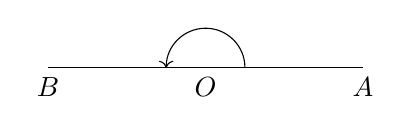
\begin{tikzpicture}
                \coordinate(A)at(2,0);
                \coordinate(O)at(0,0);
                \coordinate(B)at(-2,0);
                \draw(B)--(O)--(A);
                \tkzMarkAngle[mark=none,size=0.5cm,->](A,O,B)
                \tkzLabelPoints[below](A,B,O)
            \end{tikzpicture}
        }
    \end{minipage}
    \medskip
    \begin{minipage}[b]{.5\linewidth}
        \centering
        \subfigure[周角]{
            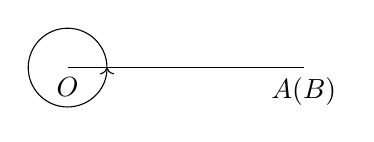
\begin{tikzpicture}
                \coordinate(A)at(3,0);
                \coordinate(O)at(0,0);
                \coordinate(B)at(1.99,-0.001);
                \draw(O)--(A);
                \tkzMarkAngle[mark=none,size=0.5cm,->](A,O,B)
                \tkzLabelPoints[below](O)
                \node[below]at(A){$A(B)$};
            \end{tikzpicture}
        }
    \end{minipage}
    \caption{平角和周角}
    \label{fig:st}
\end{figure}
\par $1^\circ$的$\dfrac{1}{60}$为$1$分,记作$1^\prime$,即$1^\circ=60^\prime$.
\par $1^\prime$的$\dfrac{1}{60}$为$1$秒,记作$1^{\prime\prime}$,即$1^\prime=60^{\prime\prime}$.
\section{角的比较}
\par 从一个角的顶点引出的一条射线,把这个角分成两个相等的角,这条射线叫做这个{\heiti 角的平分线}.
\begin{figure}[htbp]
    \centering
    \begin{tikzpicture}
        \coordinate(O)at(0,0);
        \coordinate(B)at(3,0);
        \coordinate(C)at($(O)!3cm!30:(B)$);
        \coordinate(A)at($(O)!3cm!30:(C)$);
        \draw(O)--(B);
        \draw(O)--(C);
        \draw(O)--(A);
        \tkzLabelPoints[left](O)
        \tkzLabelPoints[right](A,B,C)
    \end{tikzpicture}
    \caption{角的平分线.}
    \label{fig:angle-bisector}
\end{figure}
\par 如图\ref{fig:angle-bisector}所示,射线$OC$是$\angle AOB$的平分线. 这时,$\angle AOC=\angle BOC=\dfrac12\angle AOB$(或$\angle AOB=2\angle AOC=2\angle BOC$).
\section{多边形和圆的初步认识}
\par 由若干条不在同一直线上的线段首位顺次相连组成的封闭平面图形,叫做{\heiti 多边形}.
\par 多边形连接不相邻两个顶点的线段,叫做多边形的{\heiti 对角线}.
\par 各边相等、各角也相等的多边形叫做{\heiti 正多边形}.
\begin{figure}[htbp]
    \centering
    \begin{tikzpicture}[scale=.7]
        \tkzDefPoint(0,0){O}
        \tkzDefPoint(-3,0){B}
        \tkzDefCircle(O,B)
        \tkzGetLength{rB}
        \tkzDefPointOnCircle[R= angle 105 center O radius \rB]
        \tkzGetPoint{A}
        \tkzDrawCircle(O,A)
        \tkzDrawSegment(A,O)
        \tkzDrawSegment(B,O)
        \tkzDrawPoints(A,B,O)
        \tkzLabelPoints(O)
        \tkzLabelPoints[left](B)
        \tkzLabelPoints[above](A)
    \end{tikzpicture}
    \caption{圆}
    \label{fig:circle}
\end{figure}
\par 如图\ref{fig:circle}所示,平面上,一条线段绕着它固定的一个端点旋转一周,另一个端点形成的图形叫做{\heiti 圆}.固定的端点$O$称为圆心;线段$OA$称为半径.
\par 圆上任意两点$A,B$间的部分叫做{\heiti 圆弧},简称{\heiti 弧},记作$\yhu{AB\,}$,读作“圆弧$AB$”或“弧$AB$”;由一条弧$AB$和经过这条弧的端点的两条半径$OA,OB$所组成的图形叫做{\heiti 扇形};顶点在圆心的角叫做{\heiti 圆心角}.
\chapter{整式的乘除}
\section{同底数幂的乘法}
\[a^m\cdot a^n=a^{m+n}\,(m,n都是正整数).\]
\par 同底数幂相乘,底数不变,指数相加.
\section{幂的乘方与积的乘方}
\subsection{}
\[(a^m)^n=a^{mn}\,(m,n都是正整数).\]
\par 幂的乘方,底数不变,指数相乘.
\subsection{}
\[(ab)^n=a^nb^n(n是正整数).\]
\par 积的乘方等于把积的每一个因式分别乘方,再把所得的幂相乘.
\section{同底数幂的除法}
\[a^m\div a^n=a^{m-n}(a\neq 0,m,n都是正整数,且m>n).\]
\par 同底数幂相除,底数不变,指数相减.
\section{零指数幂与负整指数幂}
\subsection{}
\[a^0=1\,(a\neq 0); \]
\[a^{-p}=\dfrac{1}{a^p}\,(a\neq 0,p是正整数).\]
\par 一个不等于零的数,它的零次幂等于$1$,它的$-p\,(p是正整数)$次幂等于这个数的$p$次幂的倒数.
\subsection{引入零指数幂和负整数指数幂后,正整数指数幂的运算性质在指数是整数时仍然适用.}
\subsection{}
\par 一般地,一个小于$1$的正数可以表示为$a\times 10^n$,其中$1\leqslant a<10,n$是负整数.
\section{整式的乘法}
\subsection{}
\par 单项式与单项式相乘,把它们的系数、相同字母的幂分别相乘,其余字母连同它的指数不变,作为积的因式.
\subsection{}
\par 单项式与多项式相乘,就是根据分配律用单项式去乘多项式的每一项,再把所得的积相加.
\subsection{}
\par 多项式与多项式相乘,先用一个多项式的每一项乘另一个多项式的每一项,再把所得的积相加.
\subsection{}
\section{平方差公式}
\subsection{}
\par {\heiti 平方差公式}\[(a+b)(a-b)=a^2-b^2\]两数和与这两数差的积,等于它们的平方差.
\subsection{}
\section{完全平方公式}
\subsection{}
\[(a+b)^2=a^2+2ab+b^2\]
\par 两数和的频繁,等于它们的平方和加上它们的积的$2$倍.
\[(a-b)^2=a^2-2ab+b^2\]
\par 两数差的平方,等于它们的平方和减去它们的积的$2$倍.
\par 以上两个公式称为{\heiti 完全平方公式}.
\subsection{}
\section{整式的除法}
\subsection{}
\par 单项式除以单项式,把系数、同底数幂分别相除,作为商的因式;对于只在被除式里面含有的字母,则连同它的指数一起作为商的一个因式.
\subsection{}
\par 多项式除以单项式,先把这个多项式的每一项分别除以单项式,再把所得的商相加.
\chapter{相交线与平行线}
\section{两条直线的位置关系}
\subsection{}
\par 在同一平面内,两条直线的位置关系有相交和平行两种.
\par 若两条直线只有一个公共点,我们称这两条直线为{\heiti 相交线}.
\par 在同一平面内,不相交的两条直线叫做{\heiti 平行线}.
\begin{figure}[htbp]
    \centering
    \begin{tikzpicture}
        \tkzDefPoint(2,3){A}
        \tkzDefPoint(4,0){B}
        \tkzDefMidPoint(A,B)
        \tkzGetPoint{O}
        \tkzDefPointBy[rotation=center O angle -36](A)
        \tkzGetPoint{C}
        \tkzDefPointBy[rotation=center O angle -36](B)
        \tkzGetPoint{D}
        \tkzDrawSegments(A,B C,D)
        \tkzLabelPoints[above](A,C)
        \tkzLabelPoints[below](B,D)
        \tkzLabelPoints[left](O)
        \tkzMarkAngle[size=.7cm,mark=none](C,O,A)
        \tkzLabelAngle(C,O,A){2}
        \tkzMarkAngle[size=.7cm,mark=none](D,O,B)
        \tkzLabelAngle(D,O,B){1}
    \end{tikzpicture}
    \caption{对顶角}
    \label{fig:vertical-angles}
\end{figure}
\par 如图\ref{fig:vertical-angles}所示,直线$AB$与$CD$相交于点$O$,$\angle 1$与$\angle 2$有公共顶点$O$,它们的两边互为反向延长线,这样的两个角叫做{\heiti 对顶角}.
\par 对顶角性质: 对顶角相等.
\par 如果两个角的和是$180^\circ$,那么称这两个角互为{\heiti 补角}.
\par 类似地,如果两个角的和是$90^\circ$,那么称这两个角互为{\heiti 余角}.
\par 同角或等角的余角相等,同角或等角的补角相等.
\subsection{}
\par 两条直线相交成四个角,如果有一个角是直角,那么称这两条直线互相{\heiti 垂直},其中的一条直线叫做另一条直线的垂线,它们的交点叫做{\heiti 垂足}.
\par 通过用符号“$\perp$”表示两条直线互相垂直.如图\ref{fig:perpendicular},直线$AB$与直线$CD$垂直,记作$AB\perp CD$;如图\ref{fig:perp2},直线$l$与直线$m$垂直,记作$l\perp m$.其中,点$O$是垂足.
\begin{figure}[htbp]
    \begin{minipage}[b]{.5\linewidth}
        \centering
        \begin{tikzpicture}
            \tkzDefPoints{-2/0/A,2/0/B,0/2/C,0/-2/D}
            \tkzInterLL(A,B)(C,D)
            \tkzGetPoint{O}
            \tkzLabelPoints[below](A,B)
            \tkzLabelPoints[below left](O)
            \tkzLabelPoints[right](C,D)
            \tkzMarkRightAngle(B,O,C)
            \tkzDrawSegments(A,B C,D)
        \end{tikzpicture}
        \caption{垂直与垂足\uppercase\expandafter{\romannumeral1}}
        \label{fig:perpendicular}
    \end{minipage}
    \medskip
    \begin{minipage}[b]{.5\linewidth}
        \centering
        \begin{tikzpicture}
            \tkzDefPoints{0/0/A,4/2.9/B,0.5/4/C}
            \tkzDefLine[perpendicular=through C,K=-1](A,B)
            \tkzGetPoint{D}
            \tkzDrawSegments(A,B C,D)
            \tkzInterLL(A,B)(C,D)
            \tkzGetPoint{O}
            \tkzLabelPoints[right=3pt](O)
            \tkzMarkRightAngle(B,O,C)
            \tkzLabelSegment[pos=1,right](A,B){$m$}
            \tkzLabelSegment[pos=0,left](C,D){$l$}
        \end{tikzpicture}
        \caption{垂直与垂足\uppercase\expandafter{\romannumeral2}}
        \label{fig:perp2}
    \end{minipage}
\end{figure}
\par 平面内,过一点有且只有一条直线与已知直线垂直.
\begin{figure}[htbp]
    \centering
    \begin{tikzpicture}
        \tkzDefPoints{0/0/A,6/0/B,3.5/3.5/P}
        \tkzDefPointBy[projection=onto A--B](P)
        \tkzGetPoint{O}
        \tkzDrawSegments(A,B O,P)
        \tkzLabelSegment[pos=1,right](A,B){$l$}
        \tkzLabelPoints(O,P)
        \tkzMarkRightAngle(B,O,P)
    \end{tikzpicture}
    \caption{垂线段}
    \label{fig:perp3}
\end{figure}
\par 如图\ref{fig:perp3},点$P$是直线$l$外一点,$PO\perp l$,垂足为点$O$,线段$PO$叫做点$P$到直线$l$的{\heiti 垂线段}.
\par 直线外一点与直线上各点的连接的所有线段中,垂线段最短.
\par 在图\ref{fig:perp3}中,垂线段$PO$的长度叫做点$P$到直线$l$的距离.
\section{探索直线平行的条件}
\subsection{}
\begin{figure}[htbp]
    \centering
    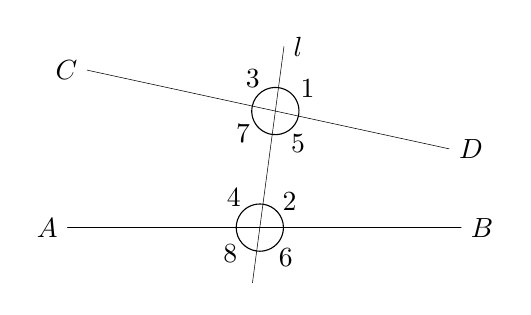
\begin{tikzpicture}
        \tkzDefPoints{0/0/A,5/0/B,0.25/2/C,4.85/1/D,2.75/2.3/E,2.35/-0.7/F}
        \tkzDrawSegments(A,B C,D E,F)
        \tkzInterLL(C,D)(E,F)
        \tkzGetPoint{G}
        \tkzInterLL(A,B)(E,F)
        \tkzGetPoint{H}
        \tkzLabelPoints[left](A,C)
        \tkzLabelPoints[right](B,D)
        \tkzLabelSegment[pos=0,right](E,F){$l$}
        \tkzMarkAngles[size=.3cm,mark=none](D,G,E B,H,G E,G,C G,H,A H,G,D F,H,B C,G,H A,H,F)
        \tkzLabelAngle[pos=.5](D,G,E){1}
        \tkzLabelAngle[pos=.5](B,H,G){2}
        \tkzLabelAngle[pos=.5](E,G,C){3}
        \tkzLabelAngle[pos=.5](G,H,A){4}
        \tkzLabelAngle[pos=.5](H,G,D){5}
        \tkzLabelAngle[pos=.5](F,H,B){6}
        \tkzLabelAngle[pos=.5](C,G,H){7}
        \tkzLabelAngle[pos=.5](A,H,F){8}
    \end{tikzpicture}
    \caption{“三线八角”}
    \label{fig:83}
\end{figure}
\par 如图\ref{fig:83},具有$\angle 1$与$\angle 2$这样的位置关系的角称为{\heiti 同位角}.
\par {\heiti 同位角相等,两直线平行.}(两条直线被第三条直线所截,如果同位角相等,那么这两直线平行.)
\par 两直线平行,用符号“$\pxx$”表示.如直线$a$与直线$b$平行,记作$a\pxx b$.
\par 过直线外一点有且只有一条直线与这条直线平行.
\par 平行于同一条直线的两条直线平行.
\par 也就是说: 如果$b\pxx a$,$c\pxx a$,那么$b\pxx c$.(如图\ref{fig:threeparallels})
\begin{figure}
    \centering
    \begin{tikzpicture}
        \tkzDefPoints{0/0/A,5/0/B,0/.5/C,5/.5/D,0/1/E,5/1/F}
        \tkzDrawSegments(A,B C,D E,F)
        \tkzLabelSegment[pos=1,right](A,B){$c$}
        \tkzLabelSegment[pos=1,right](C,D){$b$}
        \tkzLabelSegment[pos=1,right](E,F){$c$}
    \end{tikzpicture}
    \caption{平行于同一条直线的两直线平行}
    \label{fig:threeparallels}
\end{figure}
\subsection{}
\par 如图\ref{fig:83},具有$\angle 2$与$\angle 7$这样的位置关系的角称为{\heiti 内错角}; 具有$\angle 2$与$\angle 5$这样的位置关系的角称为{\heiti 同旁内角}.
\par {\heiti 内错角相等,两直线平行.\par 同旁内角互补,两直线平行.}
\par
$\begin{pmatrix}
        两条直线被第三条直线所截,如果内错角相等,那么这两直线平行. \\两条直线被第三条直线所截,如果同旁内角互补,那么这两直线平行.
    \end{pmatrix}$
\section{平行线的性质}
\subsection{}
\par {\heiti 两直线平行,同位角相等.\par 两直线平行,内错角相等.\par 两直线平行,同旁内角互补.}
\par
$\begin{pmatrix}
        两条平行直线被第三条直线所截,同位角相等. \\
        两条平行直线被第三条直线所截,内错角相等. \\
        两条平行直线被第三条直线所截,同旁内角互补.
    \end{pmatrix}$
\subsection{}
\section{用尺规作角}
\chapter{数据的收集与整理}
\section{数据的收集}
\section{普查和抽样调查}
\subsection{}
\par 为某一特定目的面对所有考察对象进行的全面调查叫做{\heiti 普查}.其中,所有考察对象的全体称为{\heiti 总体},而组成总体的每一个考察对象称为{\heiti 个体}.
\par 从总体中抽取部分个体进行调查,这种调查称为{\heiti 抽样调查},其中从总体抽取的一部分个体叫做总体的一个{\heiti 样本}.
\subsection{}
\par 随机调查,就是按机会均等的原则进行调查,即总体中的每个个体被选中的可能性都相等.这样的抽样方法是一种简单随机抽样.
\section{数据的表示}
\subsection{}
\par 在扇形统计图中,每部分占总体的百分比等于该部分所对应扇形的圆心角的度数与$360^\circ$的比.
\subsection{}
\subsection{}
\subsection{}
\section{统计图的选择}
\subsection{}
\subsection{}
\chapter{变量之间的关系}
\section{用表格表示变量之间的关系}
\par {\heiti 变量}.{\heiti 因变量}随{\heiti 自变量}的变化而变化.
\par 在变化过程中数值始终不变的量叫做{\heiti 常量}.
\section{用表达式表示变量之间的关系}
\par 表达式是我们表示变量之间关系的另一种方法.利用表达式,我们可以根据任何一个自变量的值求出相应的因变量的值.
\section{用图象表示变量之间的关系}
\subsection{}
\par 图象是表示变量之间关系的又一种方法,它的特点是非常直观.
\par 在用图象表示变量之间的关系时,通常用水平方向的数轴(称为横轴)上的点表示自变量,用竖直方向的数轴(称为纵轴)上的点表示因变量.
\subsection{}
\subsection{}
\part{七年级上册}
\setcounter{chapter}{0}
\chapter{三角形}
\section{认识三角形}
\subsection{}
\par 由不在同一直线上的三条线段首位顺次相接所组成的图形叫做{\heiti 三角形}.三角形有三条边、三个内角和三个顶点.“三角形”可以用符号“$\triangle$”表示,$\triangle ABC$的三边有时也用$a,b,c$来表示.如图\ref{fig:triangle}中,顶点$A$所对的边$BC$用$a$表示,边$AC$、边$BC$分别用$b,c$来表示.
\begin{figure}[htbp]
    \centering
    \begin{tikzpicture}
        \tkzDefPoints{0/0/B,1/3/A,5/0/C}
        \tkzDrawPolygon(A,B,C)
        \tkzLabelPoints[right](C)
        \tkzLabelPoints[left](B)
        \tkzLabelPoints[above](A)
        \tkzLabelSegment[below,pos=.5](B,C){$a$}
        \tkzLabelSegment[left,pos=.5](A,B){$c$}
        \tkzLabelSegment[right=.15cm,pos=.5](A,C){$b$}
    \end{tikzpicture}
    \caption{三角形}
    \label{fig:triangle}
\end{figure}
\par 三角形三个内角的和等于$180^\circ$.
\subsection{}
\par 我们可以按三角形内角的大小把三角形分为三类:
\begin{table}[h]
    \centering
    \begin{tabular}{c|c|c}
        \hline
        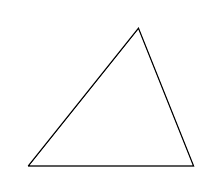
\begin{tikzpicture}[scale=.7]
            \draw (0,0)--(3,0)--(2,2.5)--(0,0);
        \end{tikzpicture}
                            &
        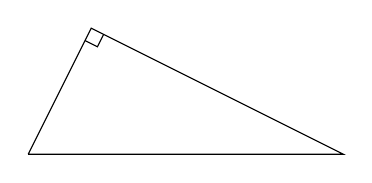
\begin{tikzpicture}[scale=.8]
            \draw (0,0) coordinate(A)--(5,0) coordinate(B)--(1,2) coordinate(C)--(0,0)
            pic [draw, angle radius=5pt, angle eccentricity=.8]{right angle = B--C--A};
        \end{tikzpicture}
                            &
        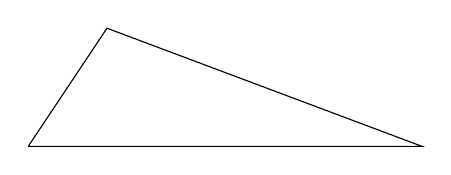
\begin{tikzpicture}
            \draw(0,0)--(5,0)--(1,1.5)--(0,0);
        \end{tikzpicture}
        \\
        \hline
        {\heiti 锐角三角形} & {\heiti 直角三角形} & {\heiti 钝角三角形} \\
        三个内角都是锐角    & 有一个内角是直角    & 有一个内角是钝角    \\
        \hline
    \end{tabular}
\end{table}
\par 通常,我们用符号“$\mathrm{Rt}\triangle ABC$”表示“直角三角形$ABC$”. 如图\ref{fig:RtABC},把直角所对应的边称为直角三角形的斜边,夹直角边的两条边称为直角边.
\begin{figure}[htbp]
    \begin{minipage}[b]{.5\linewidth}
        \centering
        \begin{tikzpicture}
            \tkzDefPoints{0/0/A,7/0/B}
            \tkzDefCircle[diameter](A,B)
            \tkzGetPoint{O}
            \tkzGetLength{rOA}
            \tkzDefPointOnCircle[R=angle 110 center O radius \rOA]
            \tkzGetPoint{C}
            \tkzDrawPolygon(A,B,C)
            \tkzMarkRightAngle(A,C,B)
            \tkzLabelPoints[right](B)
            \tkzLabelPoints[left](A)
            \tkzLabelPoints[above](C)
            \tkzLabelSegment[below](A,B){斜边}
            \tkzLabelSegment[above left](A,C){直角边}
            \tkzLabelSegment[above right](C,B){直角边}
        \end{tikzpicture}
        \caption{直角三角形}
        \label{fig:RtABC}
    \end{minipage}
    \medskip
    \begin{minipage}[b]{.5\linewidth}
        \centering
        \begin{tikzpicture}
            \tkzDefPoints{0/0/A,5/0/B,2.5/5/C}
            \tkzDrawPolygon(A,B,C)
            \tkzLabelSegment[below](A,B){底边}
            \tkzLabelSegment[above left](A,C){腰}
            \tkzLabelSegment[above right](C,B){腰}
            \tkzMarkAngles[size=.5cm,mark=none](A,C,B B,A,C C,B,A)
            \tkzLabelAngle(A,C,B){顶角}
            \tkzLabelAngles(B,A,C C,B,A){底角}
        \end{tikzpicture}
        \caption{等腰三角形}
        \label{fig:isosceles_triangle(IT)}
    \end{minipage}
\end{figure}
\par {\heiti 直角三角形的两个锐角互余.}
\subsection{}
\par 有两边相等的三角形叫做等腰三角形,如图\ref{fig:isosceles_triangle(IT)}.
\par 三边都相等的三角形叫做等边三角形,也叫作正三角形.
\par 两条边相等的直角三角形叫做等腰直角三角形.
\par {\heiti 三角形任意两边之和大于第三边.}
\par {\heiti 三角形任意两边之差小于第三边.}
\subsection{}
\par 在三角形中,连接一个顶点与它对边中点的线段,叫做这个{\heiti 三角形的中线}. 如图\ref{fig:三角形中线},$AE$是$\triangle ABC$ 的$BC$边上的中线.
\begin{figure}[htbp]
    \begin{minipage}[b]{.5\linewidth}
        \centering
        \begin{tikzpicture}
            \tkzDefPoint(0,0){A}
            \tkzDefPoint(4,0){B}
            \tkzDefPoint(2.5,3){C}
            \tkzDrawPolygon(A,B,C)
            \tkzDefSpcTriangle[medial,name=M](A,B,C){_A,_B,_C}
            \tkzDrawSegment(C,M_C)
            \tkzLabelPoints[above](C)
            \tkzLabelPoints[below](A,B)
            \tkzLabelPoint[below](M_C){$E$}
            \tkzMarkSegment[mark=|](A,M_C)
            \tkzMarkSegment[mark=|](B,M_C)
        \end{tikzpicture}
        \caption{$BE=EC$}
        \label{fig:三角形中线}
    \end{minipage}
    \medskip
    \begin{minipage}[b]{.5\linewidth}
        \centering
        \begin{tikzpicture}
            \tkzDefPoint(0,0){A}
            \tkzDefPoint(4,0){B}
            \tkzDefPoint(2.5,3){C}
            \tkzDrawPolygon(A,B,C)
            \tkzLabelPoints[above](C)
            \tkzLabelPoints[below](A,B)
            \tkzDefSpcTriangle[in,name=I](A,B,C){_a,_b,_c}
            \tkzDrawSegment(C,I_c)
            \tkzLabelPoints[above](C)
            \tkzLabelPoints[below](A,B)
            \tkzLabelPoint[below](I_c){$D$}
            \tkzMarkAngles[size=.5cm,mark=none](A,C,I_c I_c,C,B)
            \tkzLabelAngle(A,C,I_c){1}
            \tkzLabelAngle(I_c,C,B){2}
        \end{tikzpicture}
        \caption{$\angle 1= \angle 2$}
        \label{fig:三角形角平分线}
    \end{minipage}
\end{figure}
\par {\heiti 三角形的三条中线交于一点.}  这个点叫做三角形的{\heiti 重心}.
\par 在三角形中,一个内角的角平分线与它的对边相交,这个角的顶点与交点之间的线段叫做{\heiti 三角形的角平分线}. 如图\ref{fig:三角形角平分线},$AD$ 是 $\triangle ABC$的一条角平分线.
\par {\heiti 三角形的三条角平分线交于一点.}
\subsection{}
从三角形的一个顶点向它的对边所在直线作垂线,顶点和垂线之间的线段叫做{\heiti 三角形的高线},简称{\heiti 三角形的高}.如图\ref{fig:三角形高},线段$AF$是$\triangle ABC$的$BC$边上的高.
\begin{figure}[htbp]
    \centering
    \begin{tikzpicture}
        \tkzDefPoint(0,0){A}
        \tkzDefPoint(4,0){B}
        \tkzDefPoint(2.5,3){C}
        \tkzDrawPolygon(A,B,C)
        \tkzDefSpcTriangle[orthic,name=H_](A,B,C){a,b,c}
        \tkzDrawSegment(C,H_c)
        \tkzLabelPoints[above](C)
        \tkzLabelPoints[below](A,B)
        \tkzLabelPoint[below](H_c){$F$}
        \tkzMarkRightAngle(B,H_c,C)
    \end{tikzpicture}
    \caption{}
    \label{fig:三角形高}
\end{figure}
\par {\heiti 三角形的三条高所在的直线交于一点.}
\section{图形的全等}
\par 能够完全重合的两个图形称为{\heiti 全等图形}.
\par {\heiti 全等图形的形状和大小都相同.}
\par {\heiti 全等三角形的对应边相等,对应角相等.}
\section{探索三角形全等的条件}
\par 
\end{document}